% Имя файла сохранено по запросу; фактическая головка — Audio-Technica AT-3600L.
% Сборка: latexmk -xelatex -interaction=nonstopmode -halt-on-error ne5532_ad3600l_ballanced.tex
% Расчёт: .venv/bin/python scripts/calculate_balanced_riaa.py
\documentclass[a4paper,landscape,10pt]{article}
\PassOptionsToPackage{dvipsnames}{xcolor}
\usepackage{iftex}

\ifTUTeX
\usepackage{xltxtra}

\usepackage{fontspec}
\usepackage{polyglossia}
\setmainlanguage[babelshorthands=true]{russian}
\setotherlanguage{english}

\setmainfont{Times New Roman}
\setromanfont{Times New Roman} 
\setsansfont{Arial} 
\setmonofont{Courier New} 

\newfontfamily{\cyrillicfont}{Times New Roman} 
\newfontfamily{\cyrillicfontrm}{Times New Roman}
\newfontfamily{\cyrillicfonttt}{Courier New}
\newfontfamily{\cyrillicfontsf}{Arial}

% \usepackage{unicode-math}
\usepackage{amssymb}
\usepackage{amsfonts}

\else
% For pdfTeX we must use old
% 8-bit font technologies
\usepackage[T2A]{fontenc}
\usepackage[english,russian]{babel}
\usepackage[utf8]{inputenc}
\usepackage[english, russian]{babel}

%\usepackage{newtxmath}
\usepackage{amsmath}
\usepackage{amsthm}
\usepackage{amssymb}
\usepackage{amsfonts}
%\usepackage{mathtext}
\fi

%Hyphenation rules
\usepackage{hyphenat}
\hyphenation{ма-те-ма-ти-ка вос-ста-нав-ли-вать ото-бра-жа-ют-ся сге-не-ри-ро-ван-ном сим-во-лы}
% \usepackage[english, russian]{babel}

\usepackage{graphicx}
\graphicspath{ {docs/images/} {../images/} {./images/} }

\usepackage{tikz}
\usepackage{pgfplots} % для построения графиков
\usepackage{tkz-euclide}
\pgfplotsset{compat=1.18} % версия для совместимости
\usepackage{empheq}
\usetikzlibrary{positioning, calc, intersections}

\usepackage{float}

% \usepackage{comment}

\usepackage[hidelinks]{hyperref}

\newtheorem{theorem}{Теорема}[section]
\newtheorem{corollary}{Corollary}[theorem]
\newtheorem{lemma}[theorem]{Lemma}

\addto\captionsrussian{%
  \renewcommand{\figurename}{Рис.}%
  \renewcommand{\tablename}{Табл.}%
}

\usepackage{verbatim}

\newcommand{\cg}{\textnormal{\textsl{g}}}

\usepackage[dvipsnames]{xcolor}

\usepackage[siunitx, RPvoltages, american]{circuitikzgit}
\ctikzset{
    amplifiers/fill=cyan,
    sources/fill=green!20,
    diodes/fill=white,
    resistors/fill=violet,
    grounds/scale=1.2,
}

\usepackage[margin=12mm]{geometry}
\pagestyle{empty}
\setlength{\parindent}{0pt}
\ctikzset{amplifiers/fill=cyan!8,resistors/fill=white,
  grounds/scale=0.65,bipoles/length=0.95cm}
\newcommand{\kohm}{\,\text{кОм}}
\newcommand{\ohm}{\,\text{Ом}}
\newcommand{\nf}{\,\text{нФ}}
\newcommand{\uf}{\,\text{мкФ}}

% #1: L/R, #2: A/B в обозначениях деталей, #3: номер входной микросхемы,
% #4/#5: цвета проводов катушки. Плюсовой вход каждого ОУ обращён наружу.
\newcommand{\frontend}[5]{%
\begin{circuitikz}[font=\small,line width=0.6pt]
  \path[use as bounding box] (-0.7,-4.8) rectangle (12.7,4.8);
  \node[font=\bfseries] at (6,4.65) {#1: U#3 — NE5532};
  \node[op amp,noinv input up] (P) at (8.3,3) {U#3A};
  \node[op amp,noinv input down] (M) at (8.3,-3) {U#3B};
  \coordinate (IP) at (0,0 |- P.+);
  \coordinate (IM) at (0,0 |- M.+);
  \coordinate (NP) at (5.4,0 |- P.-);
  \coordinate (NM) at (5.4,0 |- M.-);
  \draw (IP) node[ocirc] {} node[above right,yshift=4pt] {$#1+$: #4}
    to[C,l_=$C_{#21}\;4.7\uf$] (3.2,0 |- P.+) -- (P.+);
  \draw (IM) node[ocirc] {} node[below right,yshift=-4pt] {$#1-$: #5}
    to[C,l=$C_{#22}\;4.7\uf$] (3.2,0 |- M.+) -- (M.+);
  \draw (3.9,0 |- P.+) node[circ] {}
    to[R] (3.9,1.8) node[ground] {};
  \draw (3.9,0 |- M.+) node[circ] {}
    to[R] (3.9,-1.8) node[ground,rotate=180] {};
  \node[anchor=east] at (3.65,2.15) {$R_{#21}\;23.5\kohm$};
  \node[anchor=east] at (3.65,-2.15) {$R_{#22}\;23.5\kohm$};
  % Дополнительная нагрузочная ёмкость — до входных разделительных C.
  \draw[gray,dashed] (0.5,0 |- P.+) node[circ] {}
    to[C] (0.5,0 |- M.+) node[circ] {};
  \node[gray,anchor=west,align=left,font=\footnotesize] at (0.85,0)
    {$C_{#29}$\\DNP};
  \draw (P.-) -- (NP) to[R] (5.4,0.4)
    to[C] (5.4,-1) node[circ] {} to[C] (NM) -- (M.-);
  \node[anchor=east,font=\footnotesize] at (5.05,1.2) {$R_{#23}\;182\ohm$};
  \node[anchor=east,align=right,font=\footnotesize] at (5.05,-0.8)
    {$C_{#23a},\;C_{#23b}$\\$1000\uf/25\text{ В}$};
  \node[font=\footnotesize] at (5.08,0.08) {$+$};
  \node[font=\footnotesize] at (5.08,-2.22) {$+$};
  % Обе обратные связи находятся между ОУ и не пересекают входные провода.
  \draw (6.3,0 |- P.-) node[circ] {} -- (6.3,1.6)
    to[R,l=$R_{#24}\;90.9\kohm$,*-*] (11,1.6) -- (11,3);
  \draw (6.3,1.6) -- (6.3,0.3)
    to[C,l=$C_{#24}\;31.5\nf$] (8.6,0.3)
    to[R,l=$R_{#26}\;10\kohm$] (11,0.3) -- (11,1.6);
  \draw (6.3,0 |- M.-) node[circ] {} -- (6.3,-1.6)
    to[R,l_=$R_{#25}\;90.9\kohm$,*-*] (11,-1.6) -- (11,-3);
  \draw (6.3,-1.6) -- (6.3,-0.3)
    to[C,l_=$C_{#25}\;31.5\nf$] (8.6,-0.3)
    to[R,l_=$R_{#27}\;10\kohm$] (11,-0.3) -- (11,-1.6);
  \draw (P.out) -- (11,3) node[circ] {} -- (12,3)
    node[ocirc] {} node[above] {$X_{#1+}$};
  \draw (M.out) -- (11,-3) node[circ] {} -- (12,-3)
    node[ocirc] {} node[below] {$X_{#1-}$};
  \node[above left,font=\footnotesize] at (P.+) {3};
  \node[below left,font=\footnotesize] at (P.-) {2};
  \node[above right,font=\footnotesize] at (P.out) {1};
  \node[below left,font=\footnotesize] at (M.+) {5};
  \node[above left,font=\footnotesize] at (M.-) {6};
  \node[below right,font=\footnotesize] at (M.out) {7};
\end{circuitikz}}

% #1: L/R; #2: A/B в обозначениях деталей и секции U3.
% Разностный фильтр: R8=R9=R10=R11, C6=C7. Знак выхода: X+ минус X-.
\newcommand{\receiver}[2]{%
\begingroup
\ifx#2A\def\pinp{3}\def\pinm{2}\def\pino{1}%
\else\def\pinp{5}\def\pinm{6}\def\pino{7}\fi
\begin{circuitikz}[font=\small,line width=0.6pt]
  \path[use as bounding box] (-0.8,-5.6) rectangle (15.7,4.7);
  \node[font=\bfseries] at (7.5,4.5) {#1: U3#2 — NE5532};
  \node[op amp,noinv input down] (U) at (8,0) {U3#2};
  \draw (0,3) node[ocirc] {} node[above right] {$X_{#1-}$}
    to[R,l=$R_{#29}\;10\kohm$] (4,3) -- (4,0 |- U.-) -- (U.-);
  \draw (0,-3) node[ocirc] {} node[below right] {$X_{#1+}$}
    to[R,l_=$R_{#28}\;10\kohm$] (4,-3) -- (4,0 |- U.+) -- (U.+);
  \draw (6,0 |- U.-) node[circ] {} -- (6,2)
    to[R,l_=$R_{#210}\;10\kohm$,*-*] (10,2) -- (10,0);
  \draw (6,2) -- (6,3.5) to[C,l=$C_{#26}\;7.5\nf$] (10,3.5) -- (10,2);
  \draw (4,0 |- U.+) node[circ] {} -- (1,0 |- U.+)
    to[C,l=$C_{#27}\;7.5\nf$] (1,-2.1) node[ground] {};
  \draw (6,0 |- U.+) node[circ] {}
    to[R,l=$R_{#211}\;10\kohm$] (6,-4.8) node[ground] {};
  \draw (U.out) -- (10,0) node[circ] {}
    to[R,l_=$R_{#212}\;100\ohm$] (11.7,0)
    to[C,l=$C_{#28}\;4.7\uf$] (14,0) -- (15,0)
    node[ocirc] {} node[above] {OUT #1};
  \draw (14,0) node[circ] {} to[R,l_=$R_{#213}\;100\kohm$]
    (14,-3.5) node[ground] {};
  \draw (15,-3.5) node[ocirc] {} -- (15,-4.3) node[ground] {};
  \node[right] at (15,-3.5) {GND};
  \node[below left,font=\footnotesize] at (U.+) {\pinp};
  \node[above left,font=\footnotesize] at (U.-) {\pinm};
  \node[above right,font=\footnotesize] at (U.out) {\pino};
\end{circuitikz}%
\endgroup}

% Развязка на КАЖДЫЙ из трёх корпусов, а не на каждую секцию ОУ.
\newcommand{\decoupling}{%
\begin{circuitikz}[font=\small,line width=0.6pt]
  \path[use as bounding box] (-0.5,-3.8) rectangle (12.8,3.0);
  \node[draw,fill=cyan!8,minimum width=1.8cm,minimum height=2.2cm,align=center]
    (U) at (10.5,0) {U$k$\\NE5532};
  \draw (0,2) node[ocirc] {} node[above right] {$+12$ В}
    -- (10.5,2) -- (U.north) node[above right] {8};
  \draw (0,0) node[ocirc] {} node[above right] {GND}
    -- (8,0) node[ground] {};
  \draw (0,-2) node[ocirc] {} node[below right] {$-12$ В}
    -- (10.5,-2) -- (U.south) node[below right] {4};
  \draw (3,2) node[circ] {} to[C,l_=$C_{Dk1}\;47\uf$] (3,0)
    node[circ] {} to[C,l_=$C_{Dk2}\;47\uf$] (3,-2) node[circ] {};
  \draw (6.5,2) node[circ] {} to[C,l=$C_{Dk3}\;100\nf$] (6.5,0)
    node[circ] {} to[C,l=$C_{Dk4}\;100\nf$] (6.5,-2) node[circ] {};
  \node at (2.6,1.5) {$+$};
  \node at (2.6,-0.6) {$+$};
  \node[align=center,font=\footnotesize] at (6,-3.2)
    {$k=1,2,3$: три одинаковых комплекта.\\100 нФ непосредственно у выводов 8 и 4.};
\end{circuitikz}}

\begin{document}
{\LARGE\bfseries AT-3600L: балансный вход, фонокорректор на трёх NE5532}\par
\vspace{2mm}
\textbf{Лист 1.} U1 — левый канал, U2 — правый.
Катушки подключены двумя сигнальными проводами каждая; L− и R− с GND не соединяются напрямую.
\begin{center}
\begin{minipage}{0.49\linewidth}
\resizebox{\linewidth}{!}{\frontend{L}{A}{1}{белый}{синий}}
\end{minipage}\hfill
\begin{minipage}{0.49\linewidth}
\resizebox{\linewidth}{!}{\frontend{R}{B}{2}{красный}{зелёный}}
\end{minipage}
\end{center}
\begin{minipage}[t]{0.48\linewidth}
\small\textbf{Вход и нагрузка головки}\par
$R_{A1}$, $R_{A2}$, $R_{B1}$, $R_{B2}$: каждый 23.5 кОм,
например два 47 кОм параллельно. Дифференциальная нагрузка катушки — 47 кОм
в рабочей полосе; резисторы одновременно задают путь входным токам ОУ.
$C_{A1}$, $C_{A2}$, $C_{B1}$, $C_{B2}$: 4.7 мкФ, плёнка, от 25 В.
\par\vspace{1mm}
$C_{A9}$, $C_{B9}$ не устанавливать по умолчанию (DNP).
Это места под дополнительную нагрузочную ёмкость, выбранную с учётом кабеля,
паразитных ёмкостей монтажа и паспорта головки.
Экран кабеля и корпус тонарма — отдельные соединения с землёй/шасси.
До подключения проверить отсутствие перемычек L−/R−/экран в тонарме и разъёмах.
Также проверить связь контактов самой головки с её корпусом и креплением.
\end{minipage}\hfill
\begin{minipage}[t]{0.48\linewidth}
\small\textbf{Первая часть RIAA и внутренние точки}\par
$R_{A3}$, $R_{B3}$: 182 Ом (можно два 91 Ом последовательно);
$C_{A3a}$/$C_{A3b}$ и $C_{B3a}$/$C_{B3b}$: по два обычных
алюминиевых электролита 1000 мкФ / 25 В на канал, \textbf{минусами вместе}.
Средняя точка каждой пары плавающая, с GND не соединяется.
Эквивалентная ёмкость — около 500 мкФ; знаки «+» показывают внешние положительные выводы.
Для обеих пар обратной связи: 90.9 кОм, 10 кОм и 31.5 нФ;
31.5 нФ можно составить из 30 нФ + 1.5 нФ параллельно.
Резисторы 0.1\%; плёночные конденсаторы согласовать между плечами, желательно до 0.5\%.
\par\vspace{1mm}
$X_{L+}$/$X_{L-}$ и $X_{R+}$/$X_{R-}$ — \textbf{внутренние} точки к листу 2.
В них ещё нет ВЧ-спада 75 мкс; это не готовые балансные линейные выходы.
В синфазном режиме входная пара имеет усиление 1, в дифференциальном —
$1+2Z_f/Z_g$. Общая коррекция завершается U3.
\end{minipage}
\vfill\footnotesize
Все земли схемы электрически общие. Питание каждой NE5532: вывод 8 — +12 В, вывод 4 — −12 В.
Номиналы с префиксами A и B относятся к разным деталям.

\newpage
{\LARGE\bfseries Разностные каскады и обычные выходы L/R}\par
\vspace{2mm}
\textbf{Лист 2.} U3A и U3B находятся в одном корпусе NE5532.
Схема сохраняет полярность: OUT $\propto V_{X+}-V_{X-}$.
\begin{center}
\begin{minipage}{0.49\linewidth}
\resizebox{\linewidth}{!}{\receiver{L}{A}}
\end{minipage}\hfill
\begin{minipage}{0.49\linewidth}
\resizebox{\linewidth}{!}{\receiver{R}{B}}
\end{minipage}
\end{center}
\begin{minipage}[t]{0.48\linewidth}
\small\textbf{Согласование разностного фильтра}\par
$R_{A8}\ldots R_{A11}$ и $R_{B8}\ldots R_{B11}$: 10 кОм, 0.1\%,
желательно согласованные резисторные сборки.
$C_{A6}=C_{A7}$ и $C_{B6}=C_{B7}$: 7.5 нФ, плёнка или C0G;
подбирать внутри каждой пары, желательно до 0.5\% или лучше.
От согласования отношений RC зависит подавление синфазного сигнала.
\par\vspace{1mm}
Каждый каскад одновременно вычитает сигналы плеч и реализует
$H_2(s)=1/(1+s\cdot75\,\text{мкс})$, поскольку $10\kohm\cdot7.5\nf=75$ мкс.
Связи от выходов U1/U2 к U3 вести парами, вдали от входов головки.
\end{minipage}\hfill
\begin{minipage}[t]{0.48\linewidth}
\small\textbf{Выход и расчётные параметры}\par
$R_{A12}$, $R_{B12}$: 100 Ом; $R_{A13}$, $R_{B13}$: 100 кОм;
$C_{A8}$, $C_{B8}$: 4.7 мкФ, плёнка, от 25 В.
Обратная связь U3 берётся \textbf{до} 100 Ом и разделительного конденсатора.
Выходы — на AUX/LINE или согласующий входной каскад АЦП, нагрузка от 47 кОм.
Прямое подключение к произвольному АЦП требует проверки его уровня и смещения.
\par\vspace{1mm}
При нагрузке 47 кОм: усиление на 1 кГц около 100.72 (40.06 дБ);
4 мВ между выводами катушки дают около 0.403 В на линейном выходе.
Расчётная ошибка RIAA, нормированная на 1 кГц, от −0.069 до +0.002 дБ
в полосе 20 Гц–20 кГц. Это результат идеальной модели, без импеданса головки,
допусков деталей и паразитных связей. Гарантированный CMRR этим не задаётся.
\end{minipage}
\vfill\footnotesize
Это новая топология, а не удвоение исходного небалансного фонокорректора.
Не добавлять к её выходу прежнюю цепь 750 Ом / 100 нФ: полюс 75 мкс уже реализован U3.

\newpage
{\LARGE\bfseries Питание, монтаж и воспроизводимый расчёт}\par
\vspace{3mm}
\begin{minipage}[t]{0.54\linewidth}
\textbf{Развязка каждого корпуса U1, U2, U3}\par
\resizebox{\linewidth}{!}{\decoupling}
\small
$C_{Dk1}$/$C_{Dk2}$: 47 мкФ, 25 В, алюминиевые электролиты;
у отрицательной шины положительная обкладка направлена к GND.
$C_{Dk3}$/$C_{Dk4}$: 100 нФ, керамика, от 25 В.
Обозначения означают $C_{D11}\ldots C_{D14}$ для U1,
$C_{D21}\ldots C_{D24}$ для U2 и $C_{D31}\ldots C_{D34}$ для U3.
\par\vspace{2mm}
\textbf{Источник ±12 В}\par
Для трёх корпусов закладываем \textbf{60 мА на плечо} внешней нагрузки,
сверх тока делителей LM317/LM337. В даташите TI максимальный ток покоя —
16 мА на корпус: три корпуса могут потребовать 48 мА ещё до выходной нагрузки.
Ток не нужно повторно удваивать при расчёте отдельного плеча.
Источник из \texttt{analog\_power\_lm317\_lm337.tex} пересчитан на этот бюджет;
при фактических напряжениях проверить запас стабилизации и нагрев.
\par\vspace{2mm}
\textbf{Плата и подключение}\par
Обе жилы каждой катушки вести рядом/витой парой с отдельным экраном.
Земля тонарма и экраны не заменяют L−/R−. Входные разъёмы изолировать от шасси.
Локальные входные земли и элементы RIAA держать вдали от токов выпрямителя.
Трансформатор и двигатель могут наводить разностный сигнал прямо в катушки;
балансный вход такую помеху не подавляет.
Линейные стабилизаторы можно разместить на этой плате, выделив им отдельную область.
\end{minipage}\hfill
\begin{minipage}[t]{0.43\linewidth}
\small\textbf{Скрипт расчёта}\par
\texttt{scripts/calculate\_balanced\_riaa.py}; общая узловая модель и графики —
\texttt{scripts/riaa\_common.py}. Номиналы читаются из секции
\texttt{[balanced]} файла \texttt{config.toml}; условия расчёта — из
\texttt{[analysis]}, \texttt{[opamp]} и \texttt{[riaa]}.
Зависимости NumPy и Matplotlib указаны в \texttt{pyproject.toml}.
\par\vspace{1mm}
Установка: \texttt{.venv/bin/python -m pip install -e .}\par
Запуск из каталога проекта:\par
{\footnotesize\ttfamily .venv/bin/python scripts/calculate\_balanced\_riaa.py}\par
Параметры запуска: \texttt{--config PATH}, \texttt{--output-dir DIR}.
Изменение TOML не переписывает номиналы на схеме автоматически.
\par\vspace{2mm}
Для частотной переменной $s=j2\pi f$ используем:
\[
 Z_f=\left(\frac1{90.9\kohm}
       +\frac1{10\kohm+\frac1{s\,31.5\nf}}\right)^{-1}.
\]
\[
 Z_g=182\ohm+\frac1{s\,500\uf},\qquad
 H_2(s)=\frac1{1+s\,75\,\text{мкс}}.
\]
\[
 H(s)=H_{\mathrm{in}}(s)
 \left(1+\frac{2Z_f}{Z_g}\right)H_2(s)H_{\mathrm{out}}(s).
\]
Для пары электролитов $C_{\mathrm{экв}}=C_aC_b/(C_a+C_b)$;
два по 1000 мкФ дают 500 мкФ.
Входные/выходные разделительные C и параллель внешней нагрузки с 100 кОм
учтены. Скрипт независимо решает узловые уравнения и проверяет совпадение с формулой,
а также нулевой синфазный выход идеальной согласованной схемы.
\par\vspace{1mm}
Дополнительно строится учебная однополюсная модель ОУ: $A_0=10^5$, GBW = 12 МГц.
Результаты: \texttt{build/balanced\_riaa/balanced.csv},
\texttt{balanced.json}, \texttt{balanced.png}, \texttt{balanced.pdf}.
Графики показывают АЧХ и отклонение от RIAA с нормировкой на 1 кГц.
\par\vspace{2mm}
\textbf{Проверка макета}\par
Проверить питание, постоянные уровни на внутренних выходах, отсутствие генерации,
АЧХ с обратной RIAA-цепью и подавление синфазной помехи с подключённым эквивалентом
головки. Расчёт не моделирует шум, перегрузку и устойчивость реального NE5532.
Уменьшение собственного шума по сравнению с исходной схемой не гарантируется.
\end{minipage}
\vfill\footnotesize
Расчётный проект, без испытания макета.
Документация: \href{https://www.ti.com/lit/ds/symlink/ne5532.pdf}{TI NE5532};
\href{https://www.analog.com/media/en/training-seminars/tutorials/MT-063.pdf}{ADI MT-063: три ОУ};
\href{https://www.analog.com/en/resources/app-notes/an-937.html}{ADI AN-937: входные токи};
\href{https://knowledge.electrochem.org/encycl/c04-appguide.pdf}{CDE: anti-series connection}.
\newpage
{\LARGE\bfseries AC-анализ ngspice: сохранённый прогон 28.11.2026}\par
\vspace{3mm}
\begin{minipage}[t]{0.45\linewidth}
\vspace{0pt}\small
% Общие данные опубликованного прогона; это не самостоятельный документ.
% Источник: docs/simulation/ngspice-2026-11-28/report.json и run_info.json.
\textbf{Условия.} Прогон ngspice 45.2 от 28.11.2026 построен по XML KiCad:
20 Гц–20 кГц, 1003 отсчёта на канал, внешняя нагрузка 47 кОм.
Нормировка RIAA — на 1 кГц; эталон имеет постоянные времени
3180, 318 и 75 мкс. Источник сигнала идеальный дифференциальный.
\par\medskip
\textbf{Модель ОУ.} Линейное однополюсное приближение:
\[
 A(s)=\frac{A_0}{1+sA_0/(2\pi\,GBW)},\qquad
 A_0=10^5,\quad GBW=12\,\text{МГц}.
\]
В снимке KiCad сопротивления собраны до 23.51 и 90.91 кОм;
аналитическая конфигурация использует округлённые 23.5 и 90.9 кОм.
Параметры питания и выходы модели идеальны.
\par\medskip
\textbf{Результаты обоих каналов.}
\begin{center}
\begin{tabular}{@{}lr@{}}
Усиление на 1 кГц, В/В & 100.23888\\
Усиление на 1 кГц, дБ & 40.02072\\
Мин. ошибка RIAA (20 кГц), дБ & $-0.11942$\\
Макс. ошибка RIAA (382.36 Гц), дБ & $+0.00131$\\
\end{tabular}
\end{center}
При входе 4 мВ RMS между плечами выход на 1 кГц составляет
около 0.401 В RMS. AC-источники $+0.5$ и $-0.5$ В задают единичный
дифференциальный сигнал для расчёта передаточной функции;
это не проверка допустимого большого сигнала.
\par\medskip
\textbf{Как читать график.} Сверху — усиление с требуемым спадом RIAA;
в середине — фаза сигнала; снизу — отклонение формы АЧХ от эталона
после нормировки обеих характеристик на 1 кГц.
Кривые L/R совпадают из-за одинаковых номиналов и параметров модели,
без заданного разброса компонентов. Конечное усиление ОУ немного меняет
результат относительно идеального расчёта.
\par\medskip
\textbf{Границы.} Не учтены импеданс головки и кабеля, паразитные параметры
платы, шум, THD и ограничение выходного размаха. Совпадение каналов в модели
не задаёт реальное согласование или CMRR; запас устойчивости не проверен.

\end{minipage}\hfill
\begin{minipage}[t]{0.52\linewidth}
\vspace{0pt}
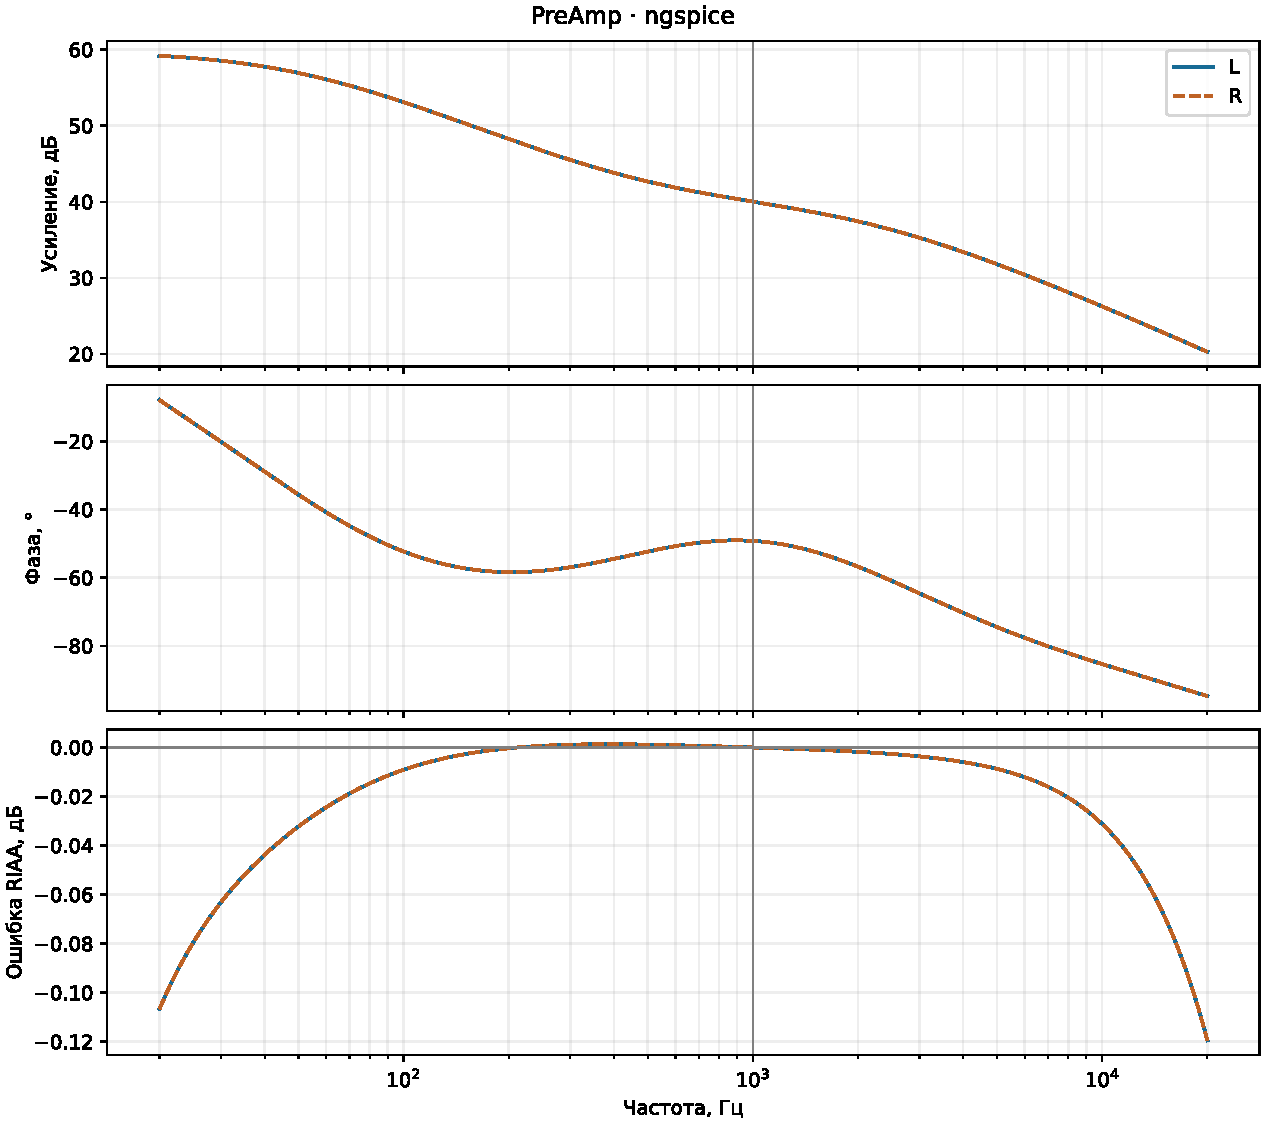
\includegraphics[width=\linewidth]{ngspice-2026-11-28-response-ru.pdf}
\small\centering
АЧХ, фаза и ошибка RIAA левого и правого каналов.
\end{minipage}
\vfill\footnotesize
Архив исходных данных и SPICE-нетлистов:
\nolinkurl{docs/simulation/ngspice-2026-11-28/}.
Графики: \nolinkurl{docs/images/}. Это симуляция, не измерение платы.
\end{document}
